
	\section{Resultados}
	Esta sessão apresenta as analises quantitativas e qualitativas dos resultados obtidos na realização dos testes descritos anteriormente.
	\\
	
	\subsubsection{Teste de latência}
	Foram coletadas as média das 1000 operações, descartando-se 10\% dos valores com maior desvio. A Tabela~\ref{tab:desvio_padrao} mostra a razão entre o desvio padrão e o valor da média para os diferentes tamanhos de arquivos testados. Apenas a maior razão entre os três níveis de RAID testados estão presentas na tabela, tanto para as operações de leitura quanto de escrita. Nota-se que a variação entre as latências foi pequena, consequentemente, os valores da média simples podem ser utilizados para realizar a comparação de desempenho. 
	\\
	
	\capstartfalse
	\begin{table} [htb]
		\caption{A taxa de desvio padrão}
		\centering
		\begin{tabular}{|l|c|c|c|c|} \hline
						& 1KB	& 100KB		& 1MB		& 10MB  \\ \hline
			desvio padão/média	& 1,7\%	& 6,7\%		& 3,7\%		& 3,1\% \\ \hline
		\end{tabular}
		\label{tab:desvio_padrao}
	\end{table}
	\capstarttrue
	
	A Figura~\ref{fig:latencia_l} representa o gráfico do teste de latência sobre a operação de leitura. Como no gráfico é difícil distinguir as linhas de cada RAID pois os valores de latência são próximos entre si, observando a Tabela~\ref{tab:latencia_l} é mais fácil notar a diferença entre os valores. Neste resultado a linha apresenta formato crescente, pois conforme o tamanho dos arquivos aumentam, o tempo gasto para concluir uma operação também aumenta. Tal característica leva ao incremento da latência observada.
	\\
	 
	De acordo com Tabela~\ref{tab:latencia_l} o RAID 1 apresenta o menor valor de latência entre todos os níveis de RAID para os arquivos de tamanho 1KB ou 100KB. Contudo, para arquivos maiores o resultado inverte, o RAID 1 apresenta a maior latência. Isso pode ser explicado pelo fato dos RAID 0 e RAID 5 necessitarem da reconstrução do arquivo a partir dos bloco de dados. A reconstrução de um arquivo pequeno é mais custosa do que sua transmissão pela rede, característica essa que tende a inverter com o aumento do arquivo.
	\\
	
	Pelos fatos acima apresentados e pelos valores da Tabela~\ref{tab:latencia_l}, é possível afirmar que na operação de leitura sobre arquivos de médio e grande porte a latência para cada nível de RAID obedece a relação de RAID 0 < RAID 5 < RAID 1.
	\\
	
	\begin{figure}[h]
		\begin{tabular}{lc}
			\begin{minipage}{.50\textwidth}
				\begin{center}
					
					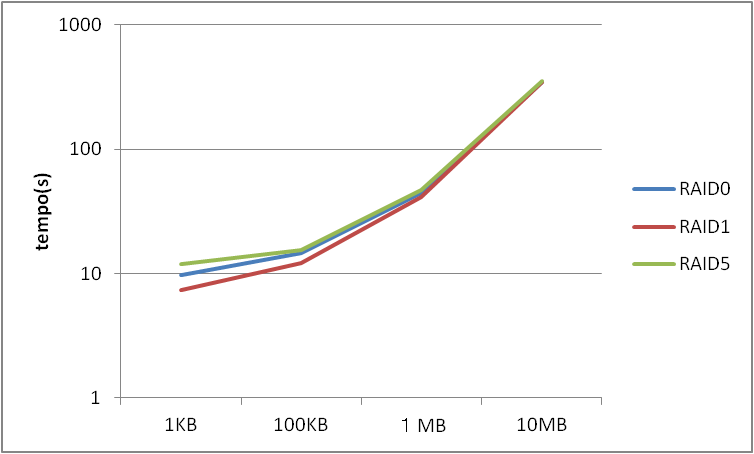
\includegraphics[clip,width=8.0cm]{images/resultados/latencia_leitura.png}
					\caption{Gráfico de latência pata leitura}
					\label{fig:latencia_l}
					
				\end{center}
				
			\end{minipage}
			
			\begin{minipage}{.5\textwidth}
				\makeatletter
				\def\@captype{table}
				\makeatother
				\caption{Tabela de latência pata leitura(s)}
				\label{tab:latencia_l}
				\begin{center}
					\begin{tabular}{|c|c|c|c|c|} \hline
								& 1KB  & 100KB & 1MB   & 10MB  \\ \hline
						RAID 0	& 9.33 & 12.26 & 38.84 & 324.73\\ \hline
						RAID 1	& 9.01 & 12.19 & 41.50 & 348.15\\ \hline
						RAID 5	& 9.76 & 12.62 & 40.11 & 326.75\\ \hline
						
						
					\end{tabular}
				\end{center}
				
			\end{minipage}
		\end{tabular}
	\end{figure}
	
	Diferente dos resultados obtidos nos testes de leitura, as diferenças entre os valores coletados sobre a operação de escrita para os três níveis de RAID são nítidas. Fato comprovado pela Figura~\ref{fig:latencia_e} e a Tabela~\ref{tab:latencia_e}.
	\\
	
	De acordo com o Gráfico~\ref{fig:latencia_e} a linha de crescimento do RAID 1 é a mais intensa. A diferença entre os outros níveis de RAID tende a aumentar caso o tamanho do arquivo também aumente.
	\\
	
	Observando apenas ao Gráfico~\ref{fig:latencia_e} têm-se a errônea sensação de que o RAID 1 possui a maior latência para qualquer tamanho de arquivo. Contudo, estudando a Tabela~\ref{tab:latencia_e} percebe-se que para os arquivos de 1KB e 100KB o RAID 5 é quem apresenta a maior latência. Isto pode ser explicado pela mesma razão do quê ocorreu no teste de leitura. Para arquivos pequenos o tempo para dividi-los em blocos é maior do que o de envia-los. A partir de 100KB, aproximadamente, a latência do RAID 1 supera o valor dos outros níveis. 
	\\
	
	Arquivos maiores do que 100KB mantém a mesma relação observada nos testes de leitura, RAID 0 < RAID 5 < RAID 1. 
	\\
	
	\begin{figure}[h]
		\begin{tabular}{lc}
			\begin{minipage}{.50\textwidth}
				\begin{center}
					
					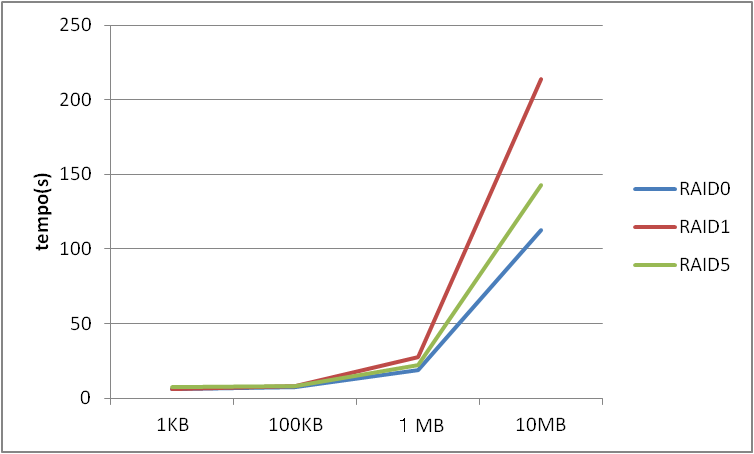
\includegraphics[clip,width=8.0cm]{images/resultados/latencia_escrita.png}
					\caption{Gráfico de latência pata escrita}
					\label{fig:latencia_e}
					
				\end{center}
				
			\end{minipage}
			
			\begin{minipage}{.5\textwidth}
				\makeatletter
				\def\@captype{table}
				\makeatother
				\caption{Tabela de latência pata escrita(s)}
				\label{tab:latencia_e}
				\begin{center}
					\begin{tabular}{|c|c|c|c|c|} \hline
								& 1KB  & 100KB & 1MB   & 10MB \\ \hline
						RAID 0	& 6.70 & 6.91 & 14.92 & 101.93\\ \hline
						RAID 1	& 6.79 & 7.53 & 23.79 & 213.94\\ \hline
						RAID 5	& 7.31 & 7.91 & 18.26 & 134.31\\ \hline
						
					\end{tabular}
					
				\end{center}
			\end{minipage}
		\end{tabular}
	\end{figure}
	
	\subsubsection{Teste de \textit{throughput}}
	Foram coletados apenas o maior valor de \textit{throughput} observado durante os testes. As linhas do gráfico possuem formato decrescente, pois o crescimento do arquivo leva ao aumento do tempo de transferência, de modo que a quantidade de operações executadas por segundo também diminuem.
	\\
	 
	
	O Gráfico~\ref{fig:throughput_l} e a Tabela~\ref{tab:throughput_l} foram obtidos ao fim dos experimentos de \textit{throughput} sobre as operações de leitura. Nota-se que o comportamento observado no teste de latência também ocorre no teste de \textit{throughput}. Pois para os arquivos de tamanhos de 1KB e 100KB, o RAID 1 apresenta os maiores valores de \textit{throughput}. Enquanto que para aquivos maiores o desempenho do RAID 1 despenca, ficando em útilmo lugar se comparado aos outros dois. A explicação para este fato pode ser a mesma do teste de latência, a relação entre os custos de reconstrução, transmissão de dados e o tamanho do arquivo.
	\\
	
	Para os arquivos maiores do que 10MB, as taxa de \textit{throughput} dos três níveis de RAID tendem a convergir para o mesmo valor, porém entre esse valor e 500KB o RAID 0 possui melhor desempenho. 
	\\
	
	\begin{figure}[h]
		\begin{tabular}{lc}
			\begin{minipage}{.50\textwidth}
				\begin{center}
					
					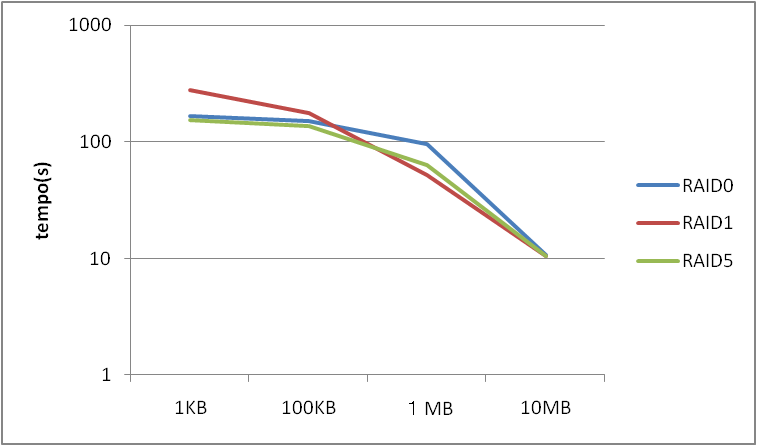
\includegraphics[clip,width=8.0cm]{images/resultados/throughput_leitura.png}
					\caption{Gráfico de throughput para leitura(ops/s)}
					\label{fig:throughput_l}
					
				\end{center}
				
			\end{minipage}
			
			\begin{minipage}{.5\textwidth}
				\makeatletter
				\def\@captype{table}
				\makeatother
				\caption{Tabela de throughput para leitura(ops/s)}
				\label{tab:throughput_l}
				\begin{center}
					\begin{tabular}{|c|c|c|c|c|} \hline
						& 1KB & 100KB & 1MB & 10MB \\ \hline
						
						RAID 0	& 167.14 & 151.63 & 95.08 & 10.63\\ \hline
						RAID 1	& 278.86 & 177.43 & 51.92 & 10.52\\ \hline
						RAID 5	& 152.79 & 135.30 & 63.34 & 10.56\\ \hline
						
					\end{tabular}
				\end{center}
				
			\end{minipage}
		\end{tabular}
	\end{figure}
	
	
	O último experimento feito é o teste de \textit{throughput} para escrita de arquivos. Diferentemente dos resultados obtidos pelos testes anteriores, em que o RAID 1 apresentava melhor desempenho apenas para os casos de arquivos pequenos, o Gráfico~\ref{fig:throughput_e} mostra que o RAID 0 apresenta a melhor taxa de \textit{throughput} desde que o arquivo não seja menor do que 1KB. Situação totalmente oposta dos testes anteriores, onde o RAID 0 apresentava bom desempenho apenas com arquivos pequenos, aqui ele apenas fraqueja lidando com arquivos pequenos. 
	\\
	
	\begin{figure}[h]
		\begin{tabular}{lc}
			\begin{minipage}{.50\textwidth}
				\begin{center}
					
					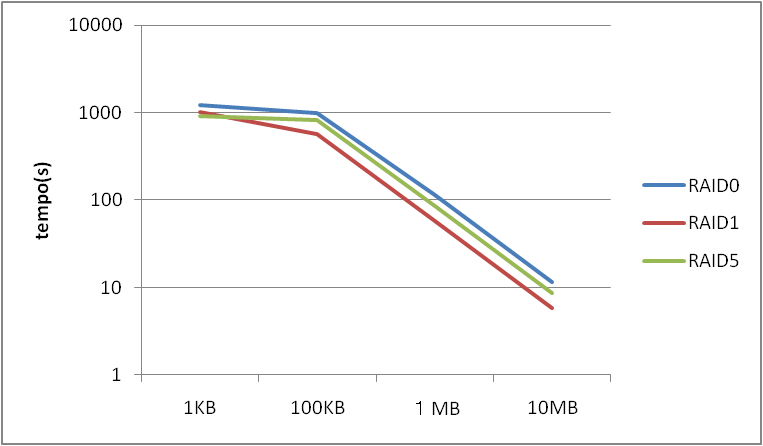
\includegraphics[clip,width=8.0cm]{images/resultados/throughput_escrita.png}
					\caption{Gráfico de throughput para escrita}
					\label{fig:throughput_e}
					
				\end{center}
				
			\end{minipage}
			
			\begin{minipage}{.5\textwidth}
				\makeatletter
				\def\@captype{table}
				\makeatother
				\caption{Tabela de throughput para escrita(ops/s)}
				\label{tab:throughput_e}
				\begin{center}
					\begin{tabular}{|c|c|c|c|c|} \hline
						& 1KB & 100KB & 1MB & 10MB \\ \hline
						
						RAID 0	& 1209.19 & 988.14 & 113.07 & 11.51\\ \hline
						RAID 1	& 1023.54 & 571.43 & 58.01  & 5.76 \\ \hline
						RAID 5	& 914.91  & 830.56 & 84.52  & 8.66 \\ \hline
						
						
					\end{tabular}
				\end{center}
				
			\end{minipage}
		\end{tabular}
	\end{figure}
	
	\section{Conclusões do Capítulo}
	
	Depois de obter os resultados dos testes foi possível verificar que o desempenho para leitura e escrita entre os três níveis de RAID respeita a relação de RAID 0 > RAID 5 > RAID 1 para a maioria dos casos. Deste modo é possível concluir que o RAID 5 agrega segurança e confiabilidade ao sistema de arquivos distribuídos com pouca degradação de desempenho, se comparado ao simples fracionamento de dados do RAID 0 ou espelhamento do RAId 1. 
	\\